\section{Diagrama de Lexis e sobrevivência na infância}

Nesta questão, foram utilizados os nascidos vivos do SINASC e os óbitos do SIM de residentes no Amapá. A análise acompanha coortes de nascimento e óbitos de menores de 5 anos, considerando o pressuposto de população fechada. Isso significa que, para fins de cálculo, não foram consideradas entradas ou saídas por migração. Essa hipótese simplifica a análise, mas deve ser interpretada com cautela, principalmente porque crianças residentes no Amapá podem se deslocar para atendimento em outros estados.

\subsection{Diagrama de Lexis}

O Diagrama de Lexis da Figura \ref{fig:lexis_ap} apresenta os óbitos de menores de 5 anos segundo ano calendário e idade aproximada ao óbito. O eixo horizontal representa o tempo calendário, o eixo vertical representa a idade e as diagonais representam as coortes de nascimento. Assim, cada diagonal acompanha uma geração ao longo do tempo.

\begin{figure}[H]
    \centering
    \caption{Diagrama de Lexis dos óbitos de menores de 5 anos. Amapá, 2000--2024.}
    
\includegraphics[width=0.95\textwidth]{imagens/lexis_ap.png}
    \label{fig:lexis_ap}
\end{figure}

\begin{figure}[H]
    \centering
    \caption{Diagrama de Lexis numérico dos óbitos de menores de 5 anos. Amapá, 2000--2024.}
    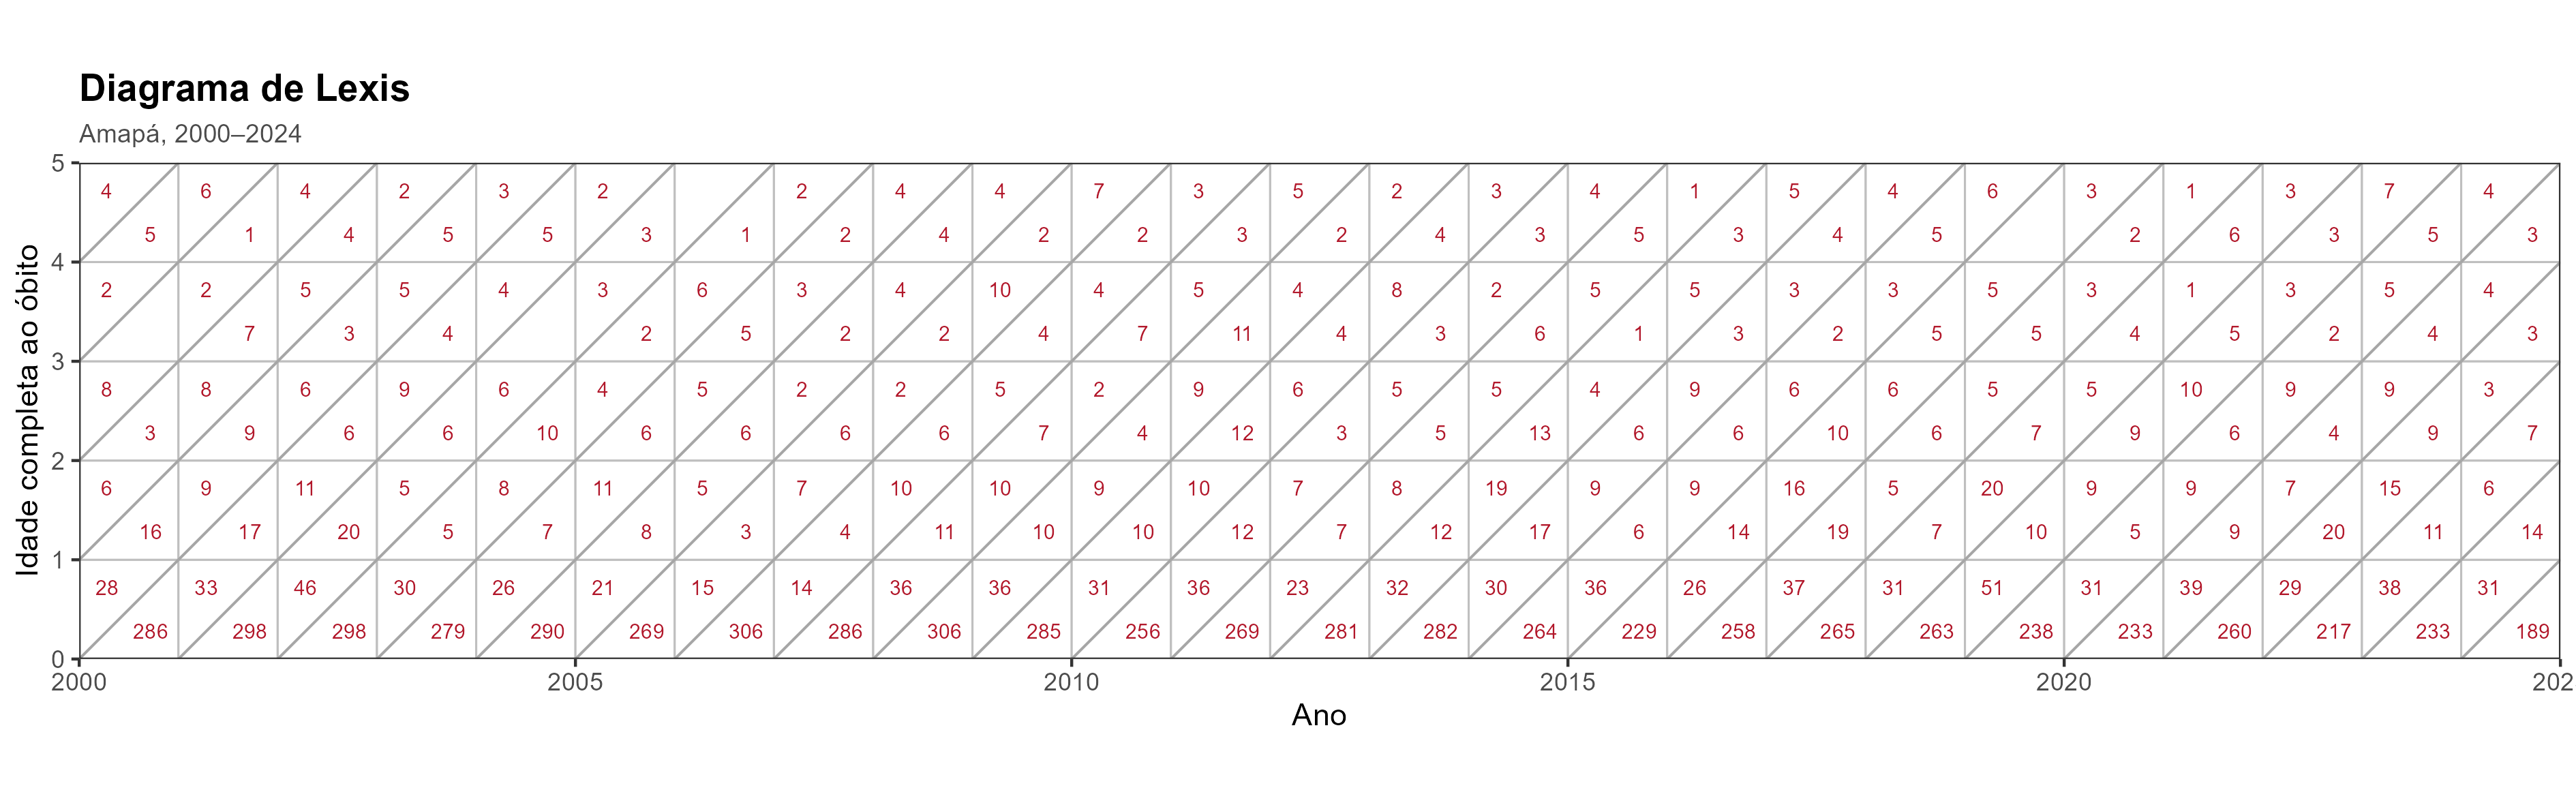
\includegraphics[width=0.95\textwidth]{imagens/lexis_ap_numerico.png}
    \label{fig:lexis_ap_num}
\end{figure}

O gráfico mostra forte concentração de óbitos abaixo de 1 ano de idade, principalmente próximos à idade zero. Esse padrão é esperado, pois o risco de morte é maior no primeiro ano de vida. Entre 1 e 4 anos, os óbitos são menos frequentes e aparecem de forma mais dispersa. A versão numérica do Lexis complementa a leitura visual ao agregar os óbitos nos quadrados idade-ano e separá-los nos triângulos correspondentes às coortes.

\subsection{Sobrevivência até a idade exata de 5 anos}

Para as coortes de nascimento de 2000 a 2019, foi calculada a probabilidade de sobreviver até a idade exata de 5 anos. As coortes posteriores não foram usadas nesse cálculo porque ainda não tinham janela completa de observação até os 5 anos.

\[
{}_{5}q_{0}(Y) = \frac{D_{0-4}(Y)}{B(Y)}
\]

\[
{}_{5}p_{0}(Y) = 1 - {}_{5}q_{0}(Y)
\]

em que $B(Y)$ representa os nascidos vivos da coorte $Y$ e $D_{0-4}(Y)$ representa os óbitos de 0 a 4 anos completos da mesma coorte. Nas tabelas, ${}_{5}q_{0}$ é apresentado por mil nascidos vivos.

\begin{figure}[H]
    \centering
    \caption{Probabilidade de sobreviver até a idade exata de 5 anos. Amapá, coortes 2000--2019.}
    
\includegraphics[width=0.85\textwidth]{imagens/grafico_5p0_ap.png}
    \label{fig:5p0_ap}
\end{figure}

\begin{table}[H]
\centering
\scriptsize
\caption{Probabilidade de sobreviver até a idade exata de 5 anos. Amapá, coortes 2000--2019.}
\label{tab:5p0_ap}
\resizebox{\textwidth}{!}{%
\begin{tabular}{rrrrr}
\toprule
\textbf{Coorte} & \textbf{Nascidos vivos} & \textbf{Óbitos 0--4} & \textbf{${}_{5}q_{0}$ por mil} & \textbf{${}_{5}p_{0}$} \\
\midrule
2000 & 14.238 & 375 & 26,3 & 0,974 \\
2001 & 14.609 & 385 & 26,4 & 0,974 \\
2002 & 14.196 & 366 & 25,8 & 0,974 \\
2003 & 14.764 & 346 & 23,4 & 0,977 \\
2004 & 13.971 & 345 & 24,7 & 0,975 \\
2005 & 14.205 & 322 & 22,7 & 0,977 \\
2006 & 14.714 & 357 & 24,3 & 0,976 \\
2007 & 14.425 & 372 & 25,8 & 0,974 \\
2008 & 15.105 & 390 & 25,8 & 0,974 \\
2009 & 14.298 & 369 & 25,8 & 0,974 \\
2010 & 15.008 & 328 & 21,9 & 0,978 \\
2011 & 15.114 & 329 & 21,8 & 0,978 \\
2012 & 14.895 & 373 & 25,0 & 0,975 \\
2013 & 15.710 & 362 & 23,0 & 0,977 \\
2014 & 16.271 & 339 & 20,8 & 0,979 \\
2015 & 15.750 & 314 & 19,9 & 0,980 \\
2016 & 15.521 & 341 & 22,0 & 0,978 \\
2017 & 15.399 & 347 & 22,5 & 0,977 \\
2018 & 15.864 & 370 & 23,3 & 0,977 \\
2019 & 15.356 & 314 & 20,4 & 0,980 \\
\bottomrule
\end{tabular}
}
\end{table}

A sobrevivência até os 5 anos permaneceu elevada em todas as coortes, variando aproximadamente entre 97,4\% e 98,0\%. Em termos complementares, a mortalidade antes dos 5 anos variou entre cerca de 19,9 e 26,4 óbitos por mil nascidos vivos. Apesar de algumas oscilações, há melhora em relação às primeiras coortes dos anos 2000.

\subsection{Sobrevivência ao primeiro aniversário}

Também foi calculada a probabilidade de sobreviver ao primeiro aniversário para as coortes de 2000 a 2023. Neste caso, foram considerados os óbitos ocorridos antes de completar 1 ano de idade.

\[
{}_{1}q_{0}(Y) = \frac{D_{<1}(Y)}{B(Y)}
\]

\[
{}_{1}p_{0}(Y) = 1 - {}_{1}q_{0}(Y)
\]

Nas tabelas, ${}_{1}q_{0}$ é apresentado por mil nascidos vivos, enquanto ${}_{1}p_{0}$ é apresentado como probabilidade.

\begin{figure}[H]
    \centering
    \caption{Probabilidade de sobreviver ao primeiro aniversário. Amapá, coortes 2000--2023.}
    
\includegraphics[width=0.85\textwidth]{imagens/grafico_1p0_ap.png}
    \label{fig:1p0_ap}
\end{figure}

\begin{table}[H]
\centering
\scriptsize
\caption{Probabilidade de sobreviver ao primeiro aniversário. Amapá, coortes 2000--2023.}
\label{tab:1p0_ap}
\resizebox{\textwidth}{!}{%
\begin{tabular}{rrrrr}
\toprule
\textbf{Coorte} & \textbf{Nascidos vivos} & \textbf{Óbitos $<1$ ano} & \textbf{${}_{1}q_{0}$ por mil} & \textbf{${}_{1}p_{0}$} \\
\midrule
2000 & 14.238 & 318 & 22,3 & 0,978 \\
2001 & 14.609 & 343 & 23,5 & 0,977 \\
2002 & 14.196 & 327 & 23,0 & 0,977 \\
2003 & 14.764 & 302 & 20,5 & 0,980 \\
2004 & 13.971 & 310 & 22,2 & 0,978 \\
2005 & 14.205 & 283 & 19,9 & 0,980 \\
2006 & 14.714 & 319 & 21,7 & 0,978 \\
2007 & 14.425 & 322 & 22,3 & 0,978 \\
2008 & 15.105 & 339 & 22,4 & 0,978 \\
2009 & 14.298 & 312 & 21,8 & 0,978 \\
2010 & 15.008 & 289 & 19,3 & 0,981 \\
2011 & 15.114 & 287 & 19,0 & 0,981 \\
2012 & 14.895 & 310 & 20,8 & 0,979 \\
2013 & 15.710 & 308 & 19,6 & 0,980 \\
2014 & 16.271 & 295 & 18,1 & 0,982 \\
2015 & 15.750 & 255 & 16,2 & 0,984 \\
2016 & 15.521 & 295 & 19,0 & 0,981 \\
2017 & 15.399 & 294 & 19,1 & 0,981 \\
2018 & 15.864 & 314 & 19,8 & 0,980 \\
2019 & 15.356 & 269 & 17,5 & 0,982 \\
2020 & 14.633 & 272 & 18,6 & 0,981 \\
2021 & 14.993 & 289 & 19,3 & 0,981 \\
2022 & 13.615 & 255 & 18,7 & 0,981 \\
2023 & 12.948 & 262 & 20,2 & 0,980 \\
\bottomrule
\end{tabular}
}
\end{table}

A comparação entre ${}_{1}q_{0}$ e ${}_{5}q_{0}$ mostra que a maior parte dos óbitos antes dos 5 anos ocorre no primeiro ano de vida. Esse resultado também aparece no Diagrama de Lexis, pela concentração de pontos na parte inferior do gráfico. A coorte de 2023 deve ser lida com atenção, pois parte dos seus óbitos antes do primeiro aniversário ocorre em 2024, ano ainda sujeito a atualização nas bases do DATASUS.

\subsection{Mortalidade antes do primeiro aniversário por raça/cor}

Para 2022 e 2023, foi calculada a probabilidade de morrer antes do primeiro aniversário segundo raça/cor. O cálculo seguiu a mesma lógica da mortalidade infantil, separando nascimentos e óbitos por categoria de raça/cor.

\[
{}_{1}q_{0,r}(Y) = \frac{D_{<1,r}(Y)}{B_{r}(Y)}
\]

em que $r$ representa a categoria de raça/cor.

\begin{figure}[H]
    \centering
    \caption{Probabilidade de morrer antes do primeiro aniversário segundo raça/cor. Amapá, coortes 2022 e 2023.}
    
\includegraphics[width=0.85\textwidth]{imagens/grafico_q0_raca_ap.png}
    \label{fig:q0_raca_ap}
\end{figure}

\begin{table}[H]
\centering
\scriptsize
\caption{Probabilidade de morrer antes do primeiro aniversário segundo raça/cor. Amapá, 2022 e 2023.}
\label{tab:q0_raca_ap}
\resizebox{\textwidth}{!}{%
\begin{tabular}{llrrrl}
\toprule
\textbf{Coorte} & \textbf{Raça/cor} & \textbf{Nascidos vivos} & \textbf{Óbitos $<1$ ano} & \textbf{${}_{1}q_{0}$ por mil} & \textbf{Observação} \\
\midrule
2022 & Branca   & 1.609  & 35  & 21,8  &  \\
2022 & Preta    & 886    & 2   & 2,3   & $n < 10$ \\
2022 & Amarela  & 22     & 2   & 90,9  & $n < 10$ \\
2022 & Parda    & 10.720 & 163 & 15,2  &  \\
2022 & Indígena & 293    & 10  & 34,1  &  \\
2022 & Ignorada & 85     & 43  & 505,9 & raça/cor ignorada \\
2023 & Branca   & 1.589  & 50  & 31,5  &  \\
2023 & Preta    & 999    & 4   & 4,0   & $n < 10$ \\
2023 & Amarela  & 35     & 0   & 0,0   & $n < 10$ \\
2023 & Parda    & 9.979  & 178 & 17,8  &  \\
2023 & Indígena & 295    & 9   & 30,5  & $n < 10$ \\
2023 & Ignorada & 51     & 21  & 411,8 & raça/cor ignorada \\
\bottomrule
\end{tabular}
}
\end{table}

Algumas categorias têm menos de 10 óbitos, o que torna as estimativas instáveis. Além disso, a categoria ignorada apresentou valores elevados, indicando problema de preenchimento e de comparabilidade entre SIM e SINASC. No período analisado, a raça/cor ignorada representou 12,4\% dos óbitos infantis no SIM e apenas 0,5\% dos nascimentos no SINASC.

Entre as categorias com maior volume de eventos, pardos apresentaram valores menores que brancos e indígenas nos dois anos analisados. Ainda assim, esses resultados devem ser lidos como uma análise exploratória, porque dependem da qualidade da informação de raça/cor e de números pequenos em algumas categorias.

\subsection{Comentários}

Os resultados da Questão 1 são coerentes entre si. O Diagrama de Lexis mostra concentração dos óbitos nos primeiros meses de vida, e as probabilidades calculadas confirmam que a maior parte da mortalidade antes dos 5 anos ocorre antes do primeiro aniversário.

A sobrevivência até 1 ano e até 5 anos é elevada nas coortes analisadas, com melhora geral em relação ao início dos anos 2000. A análise por raça/cor acrescenta uma dimensão importante, mas depende fortemente da qualidade do preenchimento das bases.

As principais limitações são o uso do pressuposto de população fechada, a possibilidade de sub-registro de óbitos e a diferença de preenchimento da raça/cor entre SINASC e SIM.
